\documentclass[UTF8]{ctexart}

\usepackage{geometry}% 版面大小
\geometry{a4paper,scale=0.7}

\usepackage{graphicx}
\usepackage{caption2}
\usepackage{subfigure}
\usepackage{float}

\usepackage[hidelinks]{hyperref}

\title{作业4}
\author{刘时宜 201180078}
\date{\today}

\begin{document}
    \maketitle
    \tableofcontents
    
    \section{编写程序并编译}
    编写运行时能按要求打印自己姓名学号以及时间的c语言程序,并使用gcc进行编译后运行以确认程序正确性,如下图所示:
    \begin{figure}[H]
        \centering
        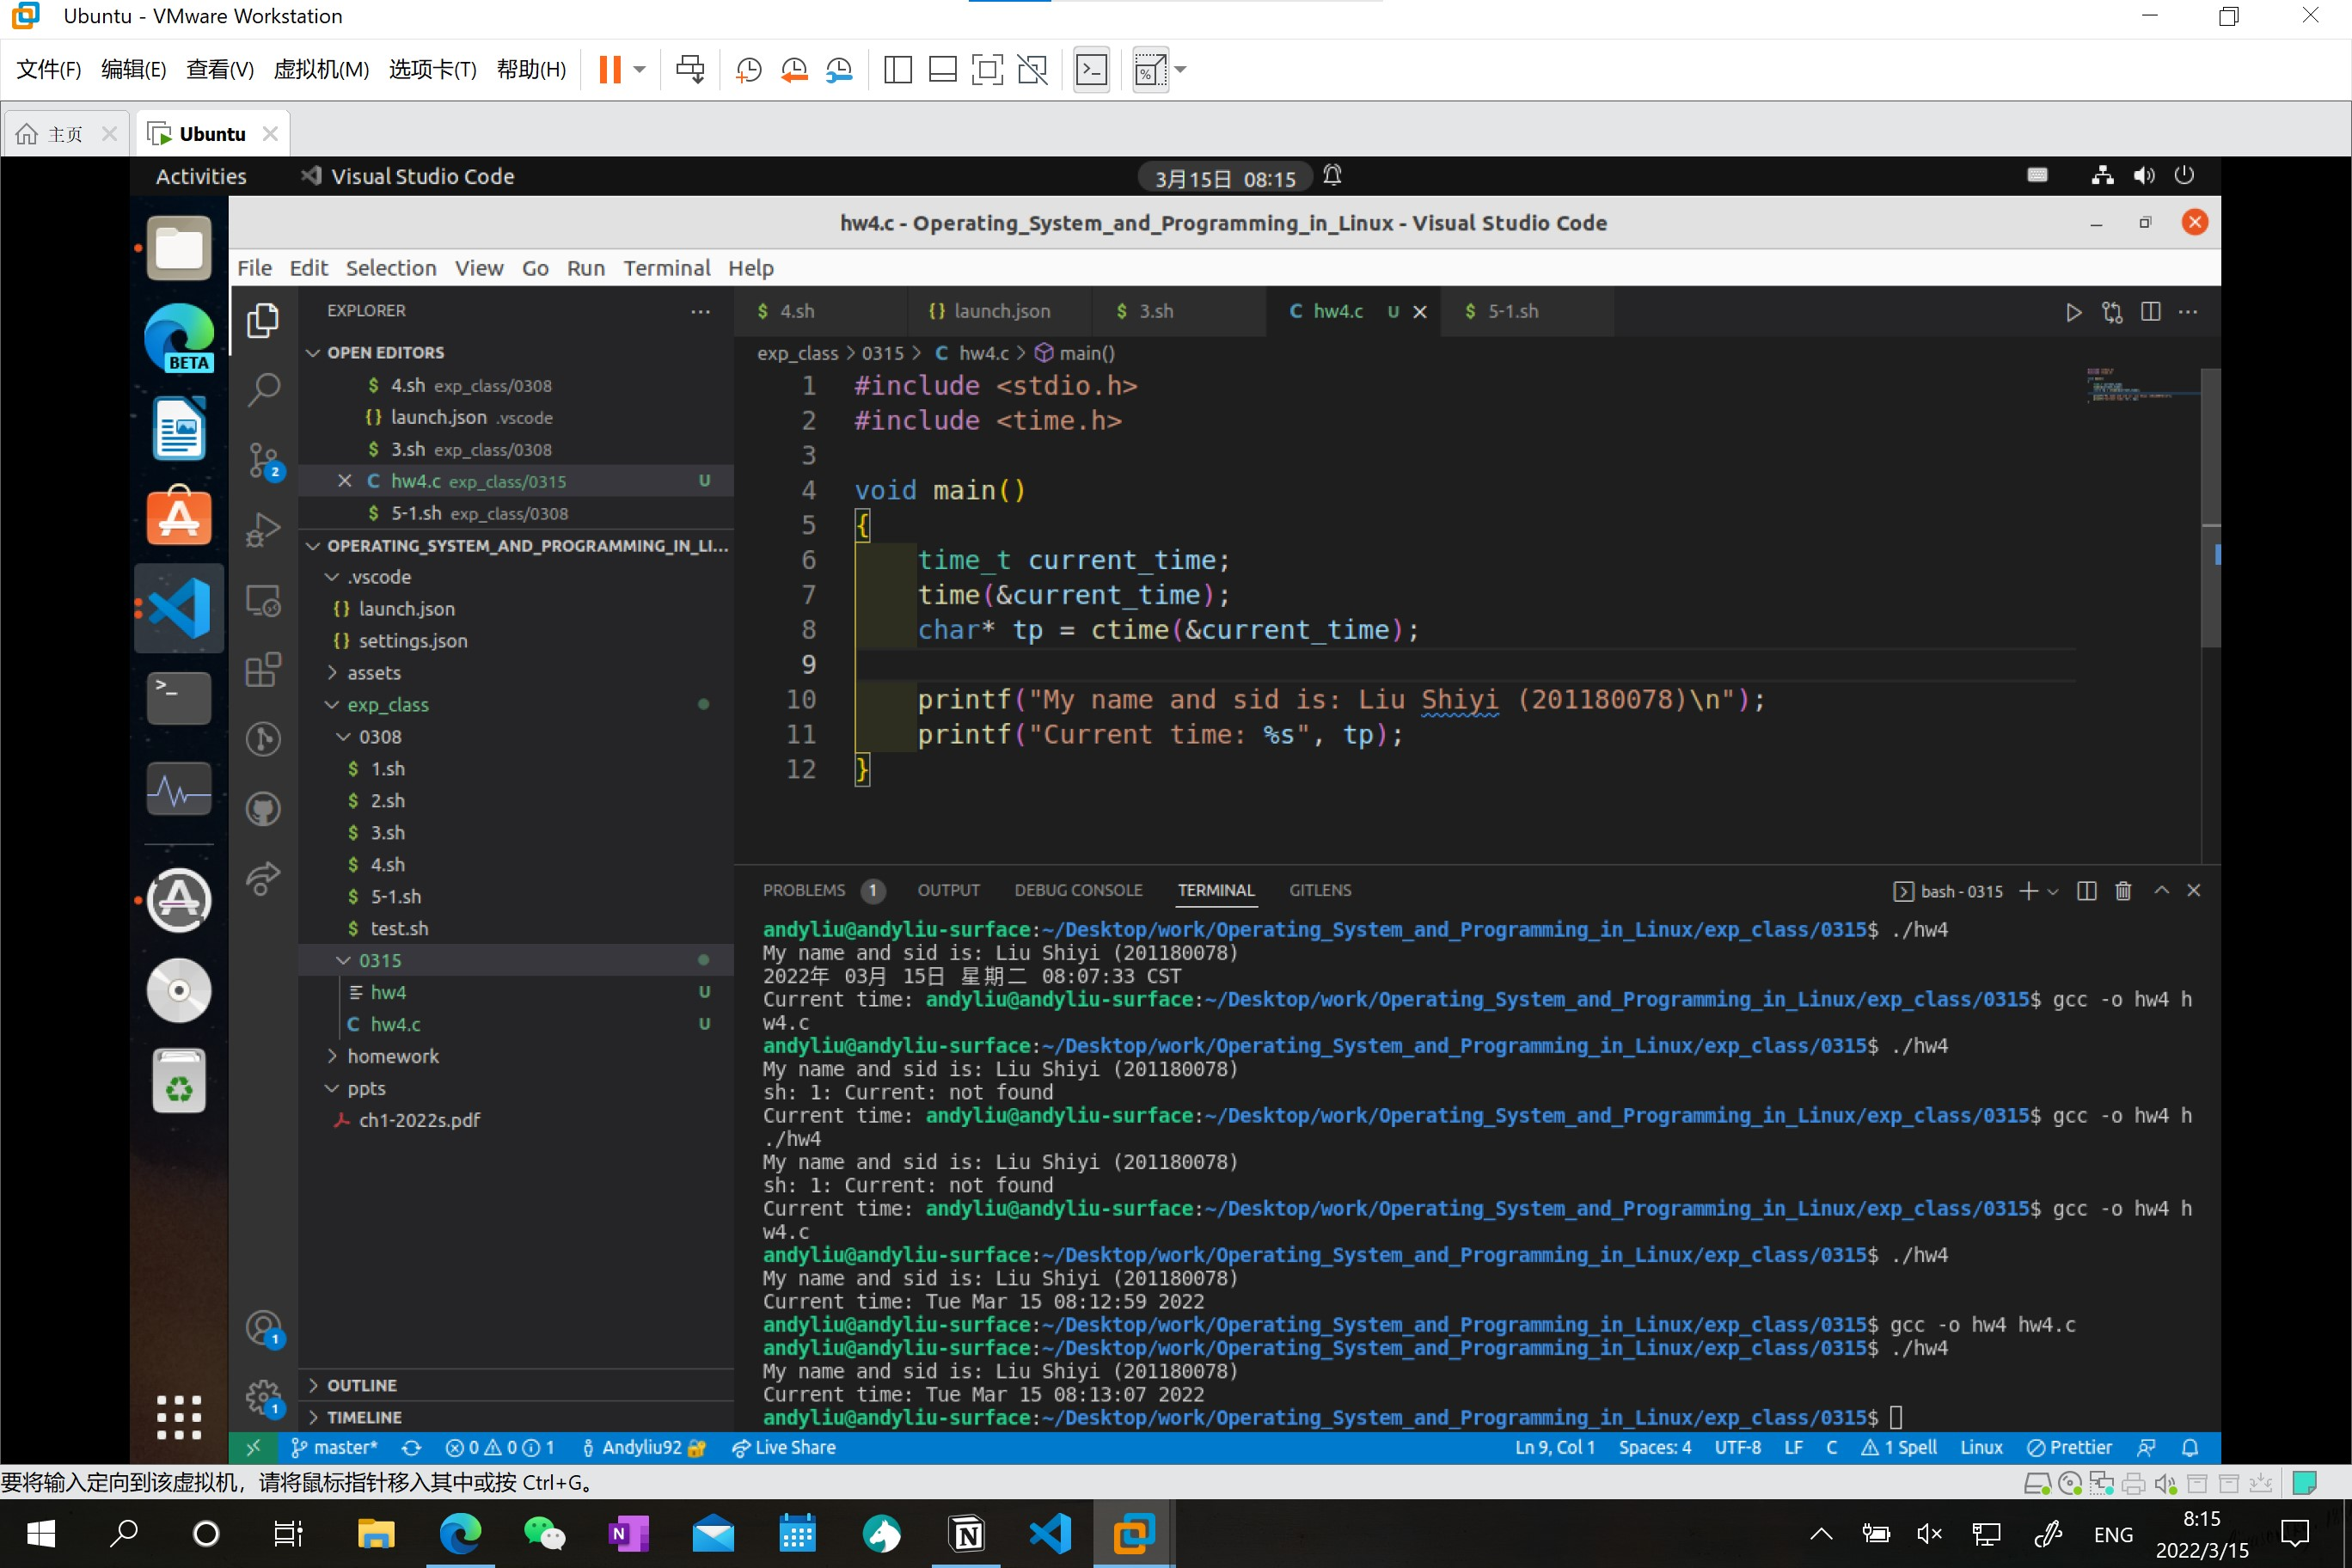
\includegraphics[width=0.8\textwidth]{assets/1.jpg}
    \end{figure}

    \section{编辑.bashrc文件}
    为了能使每次打开bash窗口时显示上述文字,在\verb|.bashrc|文件中加入一行以自动运行上面编译的程序。
    \begin{figure}[H]
        \centering
        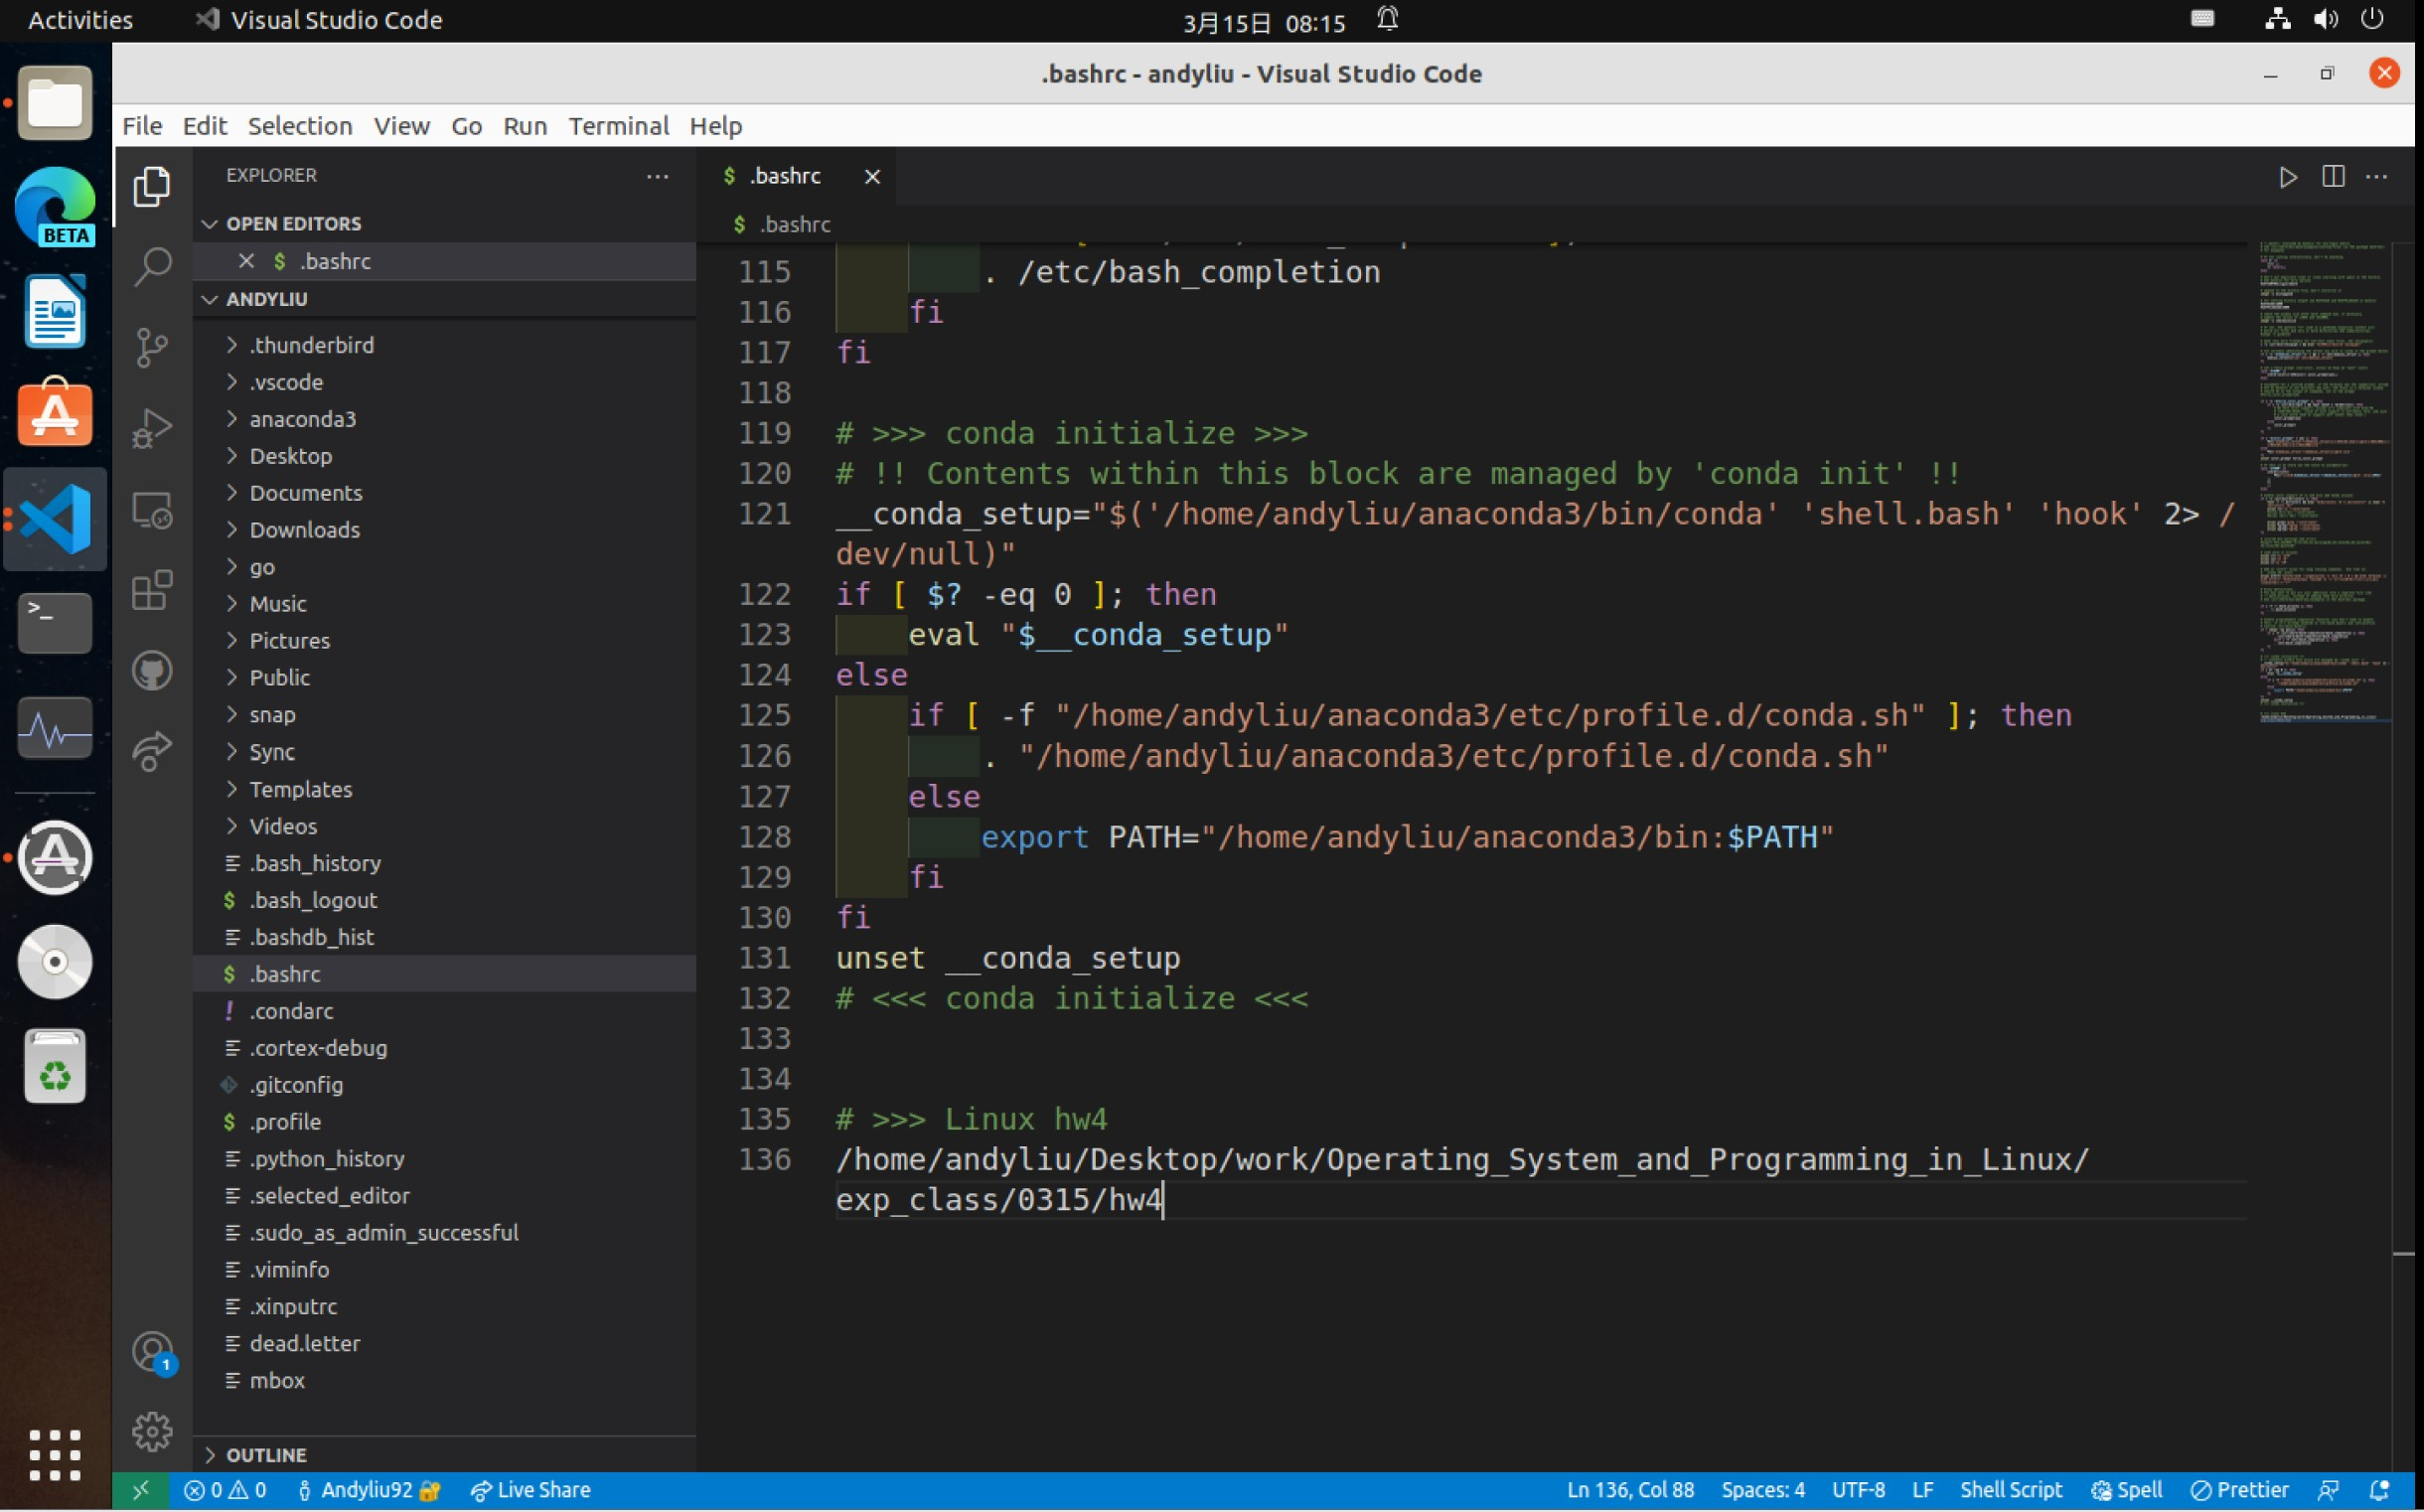
\includegraphics[width=0.8\textwidth]{assets/2.jpg}
    \end{figure}

    \section{打开bash窗口查看效果}
    可以看到,打开的新窗口显示了相应文字。
    \begin{figure}[H]
        \centering
        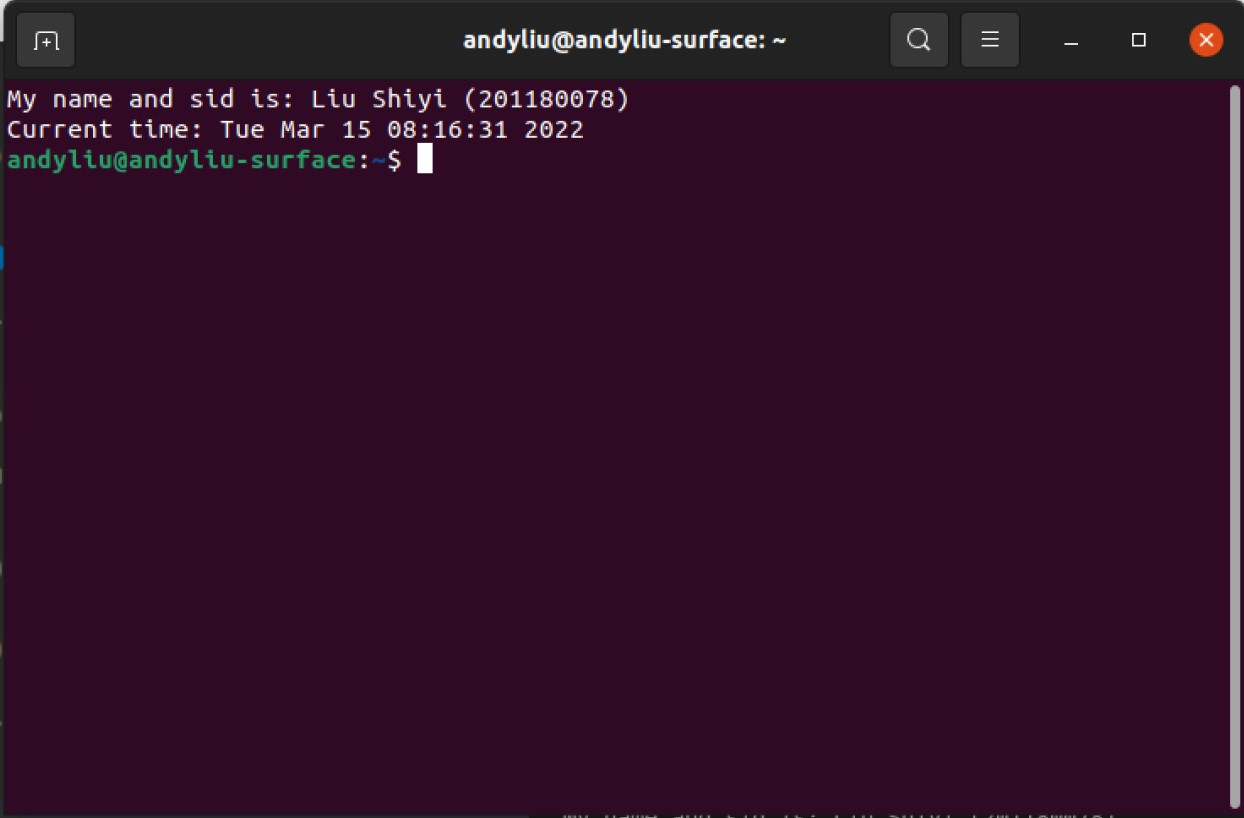
\includegraphics[width=0.8\textwidth]{assets/3.jpg}
    \end{figure}

\end{document}